\subsection{Predstavitev stroja in kosa}
Za svoj stroj sem si izbral dolgostružni avtomat Gauthier GM-127,
prikazan na Sliki \ref{gauthier_priblizano}.
Ima 5 držal za orodja in 3 gnana orodja, vidna na spodnji
Sliki \ref{gauthier_priblizano}. Omogoča struženje do ø12,7 mm.
Ima tudi možnost nadgradnje z roko za preprijem kosa pri odrezovanju in
povrtavanje ali vrezovanje navoja iz druge strani.

\begin{figure}[H]
	\begin{center}
		\includegraphics[width=8cm]{gauthier_slika.jpg}
		\caption{Krivuljni avtomat Gauthier GM-127, ki sem ga nastavljal.
			\cite{interna}}
		\label{gauthier_priblizano}
	\end{center}
\end{figure}

Za izdelek sem si izbral pušo iz materiala 1.4305.
Na Sliki \ref{delavniska_risba} je delavniška risba z
merami in tolerancami kosa. Stranki je najbolj pomembna dolžina
kosa 6,8 \(\pm\) 0,05 mm, zato se ta kasneje posebej preverja s
100 \% kontrolo. Pomemben je tudi premer izvrtine \(\phi\) 1,4 \(+\) 0,1 mm.
Premer puše \(\phi\) 5 \(\pm\) 0,05 mm je prav tako pomemben, ampak se ga
posebej ne preverja, saj je odvisen od materiala, ki je dobavljen.
Dimenzije posnetij niso pomembne, saj jih je tudi težko izmeriti,
pomembno je le, da robovi niso ostri in da nimajo srha.

\begin{figure}[H]
	\begin{center}
		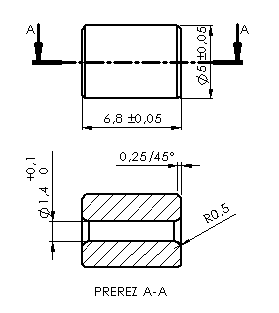
\includegraphics[width=8cm]{izdelek_risba.png}
		\caption{Risba končnika žice
			\cite{interna}}
		\label{delavniska_risba}
	\end{center}
\end{figure}

Izdelek se uporablja kot končnik žice, ki se napelje skozi
luknjo v sredini izdelka. Za lažjo napeljavo so v luknji zahtevana
posnetja v obliki radiusa. Za tem se končnik fiksira s
stiskanjem v hidravlični stiskalnici.